Podemos estudar o comportamento desse tipo de retificador através do circuito da figura \ref{fig:RTDPM}, i.e., uma associação de três retificadores monofásicos de meia onda.  Note que esse retificador opera na alimentação em uma estrutura Y, ou seja, nas tensões de fase com acesso ao neutro.

\begin{figure}[ht]
    \center
    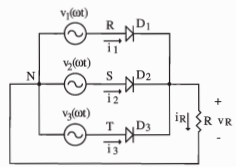
\includegraphics[scale=1.6]{imagens/RetTrifPontMed.PNG}
    \caption{Retificador trifásico a diodo com ponto médio.}\label{fig:RTDPM}
    \caption*{Fonte: Eletrônica de Potência (2006)}
\end{figure}

Nele, associamos um diodo a cada fase da alimentação, resultando nas formas de onda conforme ilustra a figura \ref{fig:FRTDPM}.

\begin{figure}[ht]
    \center
    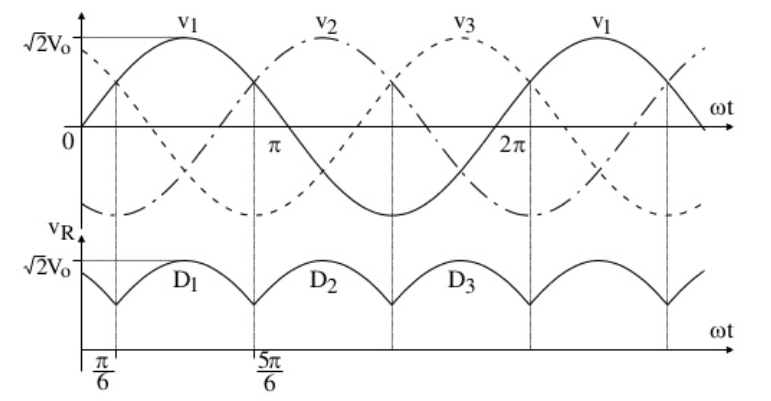
\includegraphics[scale=1]{imagens/FormasOndasRetTrifPont.PNG}
    \caption{Formas de onda para a figura \ref{fig:RTDPM}.}\label{fig:FRTDPM}
    \caption*{Fonte: Eletrônica de Potência (2006)}
\end{figure}

O valor da tensão média na carga é
\begin{align*}
V_{L,med} = \frac{3}{2\pi}{\int_{\frac{\pi}{6}}^{\frac{5\pi}{6}}}{\sqrt{2}{V_o}{\sin(\omega{t})}{d(\omega{t})}} \\
V_{L,med} = \frac{3{\sqrt{3}{\sqrt{2}}{V_o}}}{2\pi} \\
V_{L,med} = 1,17 V_o
.\end{align*}

Dessa forma, a corrente média na carga é \[
I_{L,med} = \frac{1,17 V_o}{R}
.\] 

A corrente médio nos diodos é \[
I_{D,med} = \frac{I_{L,med}}{3}
.\] 

O valor eficaz da corrente nos diodos pode ser calculado como
\begin{align*}
    I_{D,ef} &= \sqrt{\frac{1}{2\pi}{\int_{\frac{\pi}{6}}^{\frac{5\pi}{6}}}{[{\frac{\sqrt{2}{V_o}}{R}}{\sin(\omega{t})}}]^2{d(\omega{t})}} \\
	     &= 0,59{I_{Lmed}}
.\end{align*}

A expansão em série de Fourier da tensão na carga é
\begin{align*}
    V_{L}{(\omega{t})} &= 1,17{V_o} + \frac{2.1,17}{8}{V_o}{\sin(3\omega{t})} \\
    &= 1,17 V_o + 0,3V_o{\sin(3\omega{t})}
.\end{align*}
Dessa forma, a corrente na carga é \[
i_L(\omega{t}) = \frac{1,17 V_o}{R} + \frac{0,3 V_o}{\sqrt{R^2 + {9\omega^2}{L^2}}}{\sin(3\omega{t} - \phi_3)}
,\] onde \[{\phi_3} = \tan^{-1}{\frac{3\omega{t}}{R}}\]

O valor eficaz da corrente de carga pode ser calculado por \[
I_{L,ef} = \sqrt{(I_{L,med}^2 + I_{3,ef}^2)}
,\] onde $I_{L,med} = \frac{1,17 V_o}{R}$ e \[
I_{3,ef} = \frac{0,3 V_o}{\sqrt{2}{\sqrt{R^2 + 9\omega^2}{L^2}}}
.\] 
 
O valor eficaz da corrente em cada diodo (corrente eficaz de fase) é
\begin{align*}
I_{D,ef} &= \sqrt{\frac{1}{2\pi}{\int_{0}^{\frac{2\pi}{3}}}{(I_{L,med})^2}{d(\omega{t})}} \\
&= \frac{I_{L,med}}{\sqrt{3}}
.\end{align*}

O valor médio da corrente em cada diodo é definido através da corrente média da carga, i.e., \[
    I_{D,med} = \frac{I_{L,med}}{3}
.\]

Para o cálculo da tensão de pico sobre os diodos quando estes não estão conduzindo, utilizar-se-á o caso em que $D_2$ conduz a corrente da carga, como na figura \ref{fig:SEFCD}.

\begin{figure}[ht]
    \center
    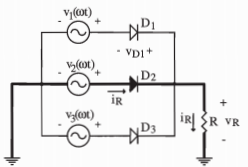
\includegraphics[scale=1.4]{imagens/SegEtapaFuncioD2.PNG}
    \caption{Segunda etapa de funcionamento do circuito.}\label{fig:SEFCD}
    \caption*{Fonte: Eletrônica de Potência (2006)}
\end{figure}

A tensão sobre o diodo $D_1$ pode ser determinada pela malha que contém $D_1$ e $D_2$, ou seja,
\begin{align*}
    \vec{V_1} + \vec{V}_{D_1} = \vec{V_2} + \vec{V_{D_2}} \\
    \implies \vec{V_{D1}} = \vec{V_2} - \vec{V_1}
.\end{align*}
Sendo $V_i$ a tensão eficaz da alimentação, então $V_{1,p} = \sqrt{2}{V_o}$ é o valor de pico da tensão de alimentação, logo \[
V_{D1p} = \sqrt{3}\sqrt{2}{V_o} \approx 2,45 V_o
.\] 


